\begin{frame}[allowframebreaks]{}
    \begin{figure}
        \centering
        \fetchconvertimage{https://blogs.mathworks.com/deep-learning/files/2021/10/BP3_fig1-1024x390.jpg}{images/gan/architecture.png}{width=1.05\textwidth,keepaspectratio}
        \caption*{Architecture of a Generative Adversarial Network (GAN). The generator creates fake data, while the discriminator distinguishes between real and fake data. The two networks are trained in opposition to each other, leading to improved performance over time.}
    \end{figure}
\end{frame}

\begin{frame}[allowframebreaks]{GANs: Motivation}
So far, we have studied generative models based on maximizing likelihood or its approximations:
\begin{enumerate}
    \item \textbf{Autoregressive Models}: $p_\theta(x) = \prod^N_{i=1} p_\theta(x_i|x_{<i})$
    \item \textbf{Variational Autoencoders (VAEs)}: $p_\theta(x) = \int_z p_\theta(x|z) p_\theta(z)$
    \item \textbf{Normalizing Flow Models}: $p_X(x;\theta) = p_Z(f_\theta^{-1}(x)) \left | \det \left( \frac{\partial f_\theta^{-1}(x)}{\partial x} \right )\right |$
\end{enumerate}

\begin{block}{Problem with Traditional Generative Models:}
    \begin{itemize}
        \item They often require complex approximations or sampling methods.
        \item They can produce blurry or unrealistic samples.
        \item They depend on explicit density estimation, which can be computationally expensive.
    \end{itemize}
\end{block}

What if we give up on explicitly modeling density, and just want
ability to sample?

\framebreak

\textbf{Generative Adversarial Networks (GANs)} provide a solution to this problem by introducing a novel approach to generative modeling:
\begin{itemize}
    \item (introduced by Ian Goodfellow et al., 2014) do not require explicit density estimation or Markov chains.
    \item consist of two neural networks—a \textbf{generator} and a \textbf{discriminator}—in a 2-player (zero-sum) game.
    \item The adversarial setup enables the generator to learn complex data distributions and produce high-fidelity, realistic samples.
\end{itemize}

\end{frame}

\begin{frame}[allowframebreaks]{GAN Progress}
    \begin{figure}
        \centering
        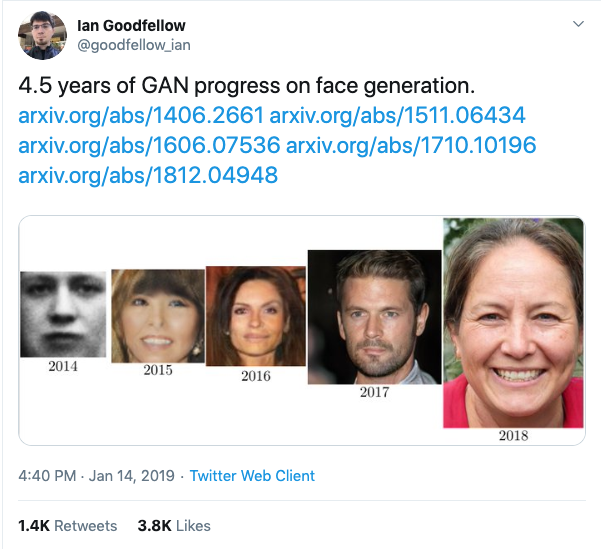
\includegraphics[height=0.8\textheight,keepaspectratio]{images/gan/motivation-1.png}
    \end{figure}
    \begin{itemize}
        \item GANs are the most prominent example of Implicit Models.
    \end{itemize}

    \framebreak

    
    \centering
    \href{https://www.youtube.com/watch?v=sW6D34mckkk}{https://www.youtube.com/watch?v=sW6D34mckkk} \\
    \vspace{2cm}
    \raggedleft
    \small [BigGAN, Brock, Donahue, Simonyan, 2018]
    

    \framebreak

    \begin{figure}
        \centering
        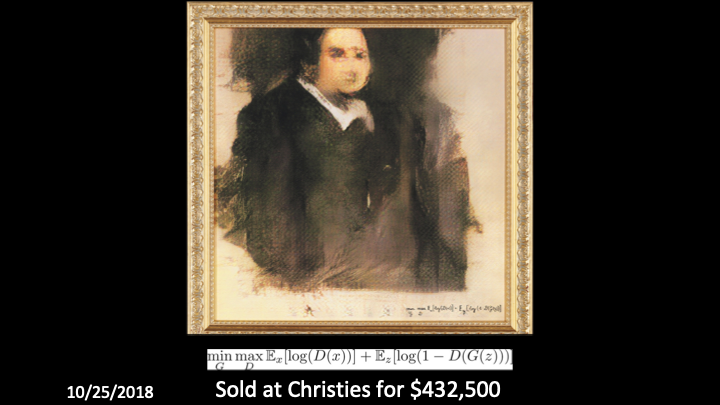
\includegraphics[height=0.9\textheight,keepaspectratio]{images/gan/motivation-2.png}
    \end{figure}
\end{frame}